\section{Durchführung}
\label{sec:Durchführung}

Für alle Versuchsreihen wird eine optische Bank verwendet, also eine Messschiene, auf der alle optischen Elemente befestigt sind und dessen absolute Positionen auf der Schiene
abgelesen werden können. Der Aufbau besteht aus einer Halogenlampe, einem weißen Schirm, verschiedenen Streu- und Sammellinsen und einer Schablone (\textit{Perl L}, Abb. \ref{fig:PerlL}), die durch
punktweise Öffnungen ein L formt. Die Schablone dient zur Erzeugung eines Bildes, welches auf dem Schirm abgebildet und scharfgestellt werden kann und als Referenzgröße dient.

\begin{figure}
    \centering
    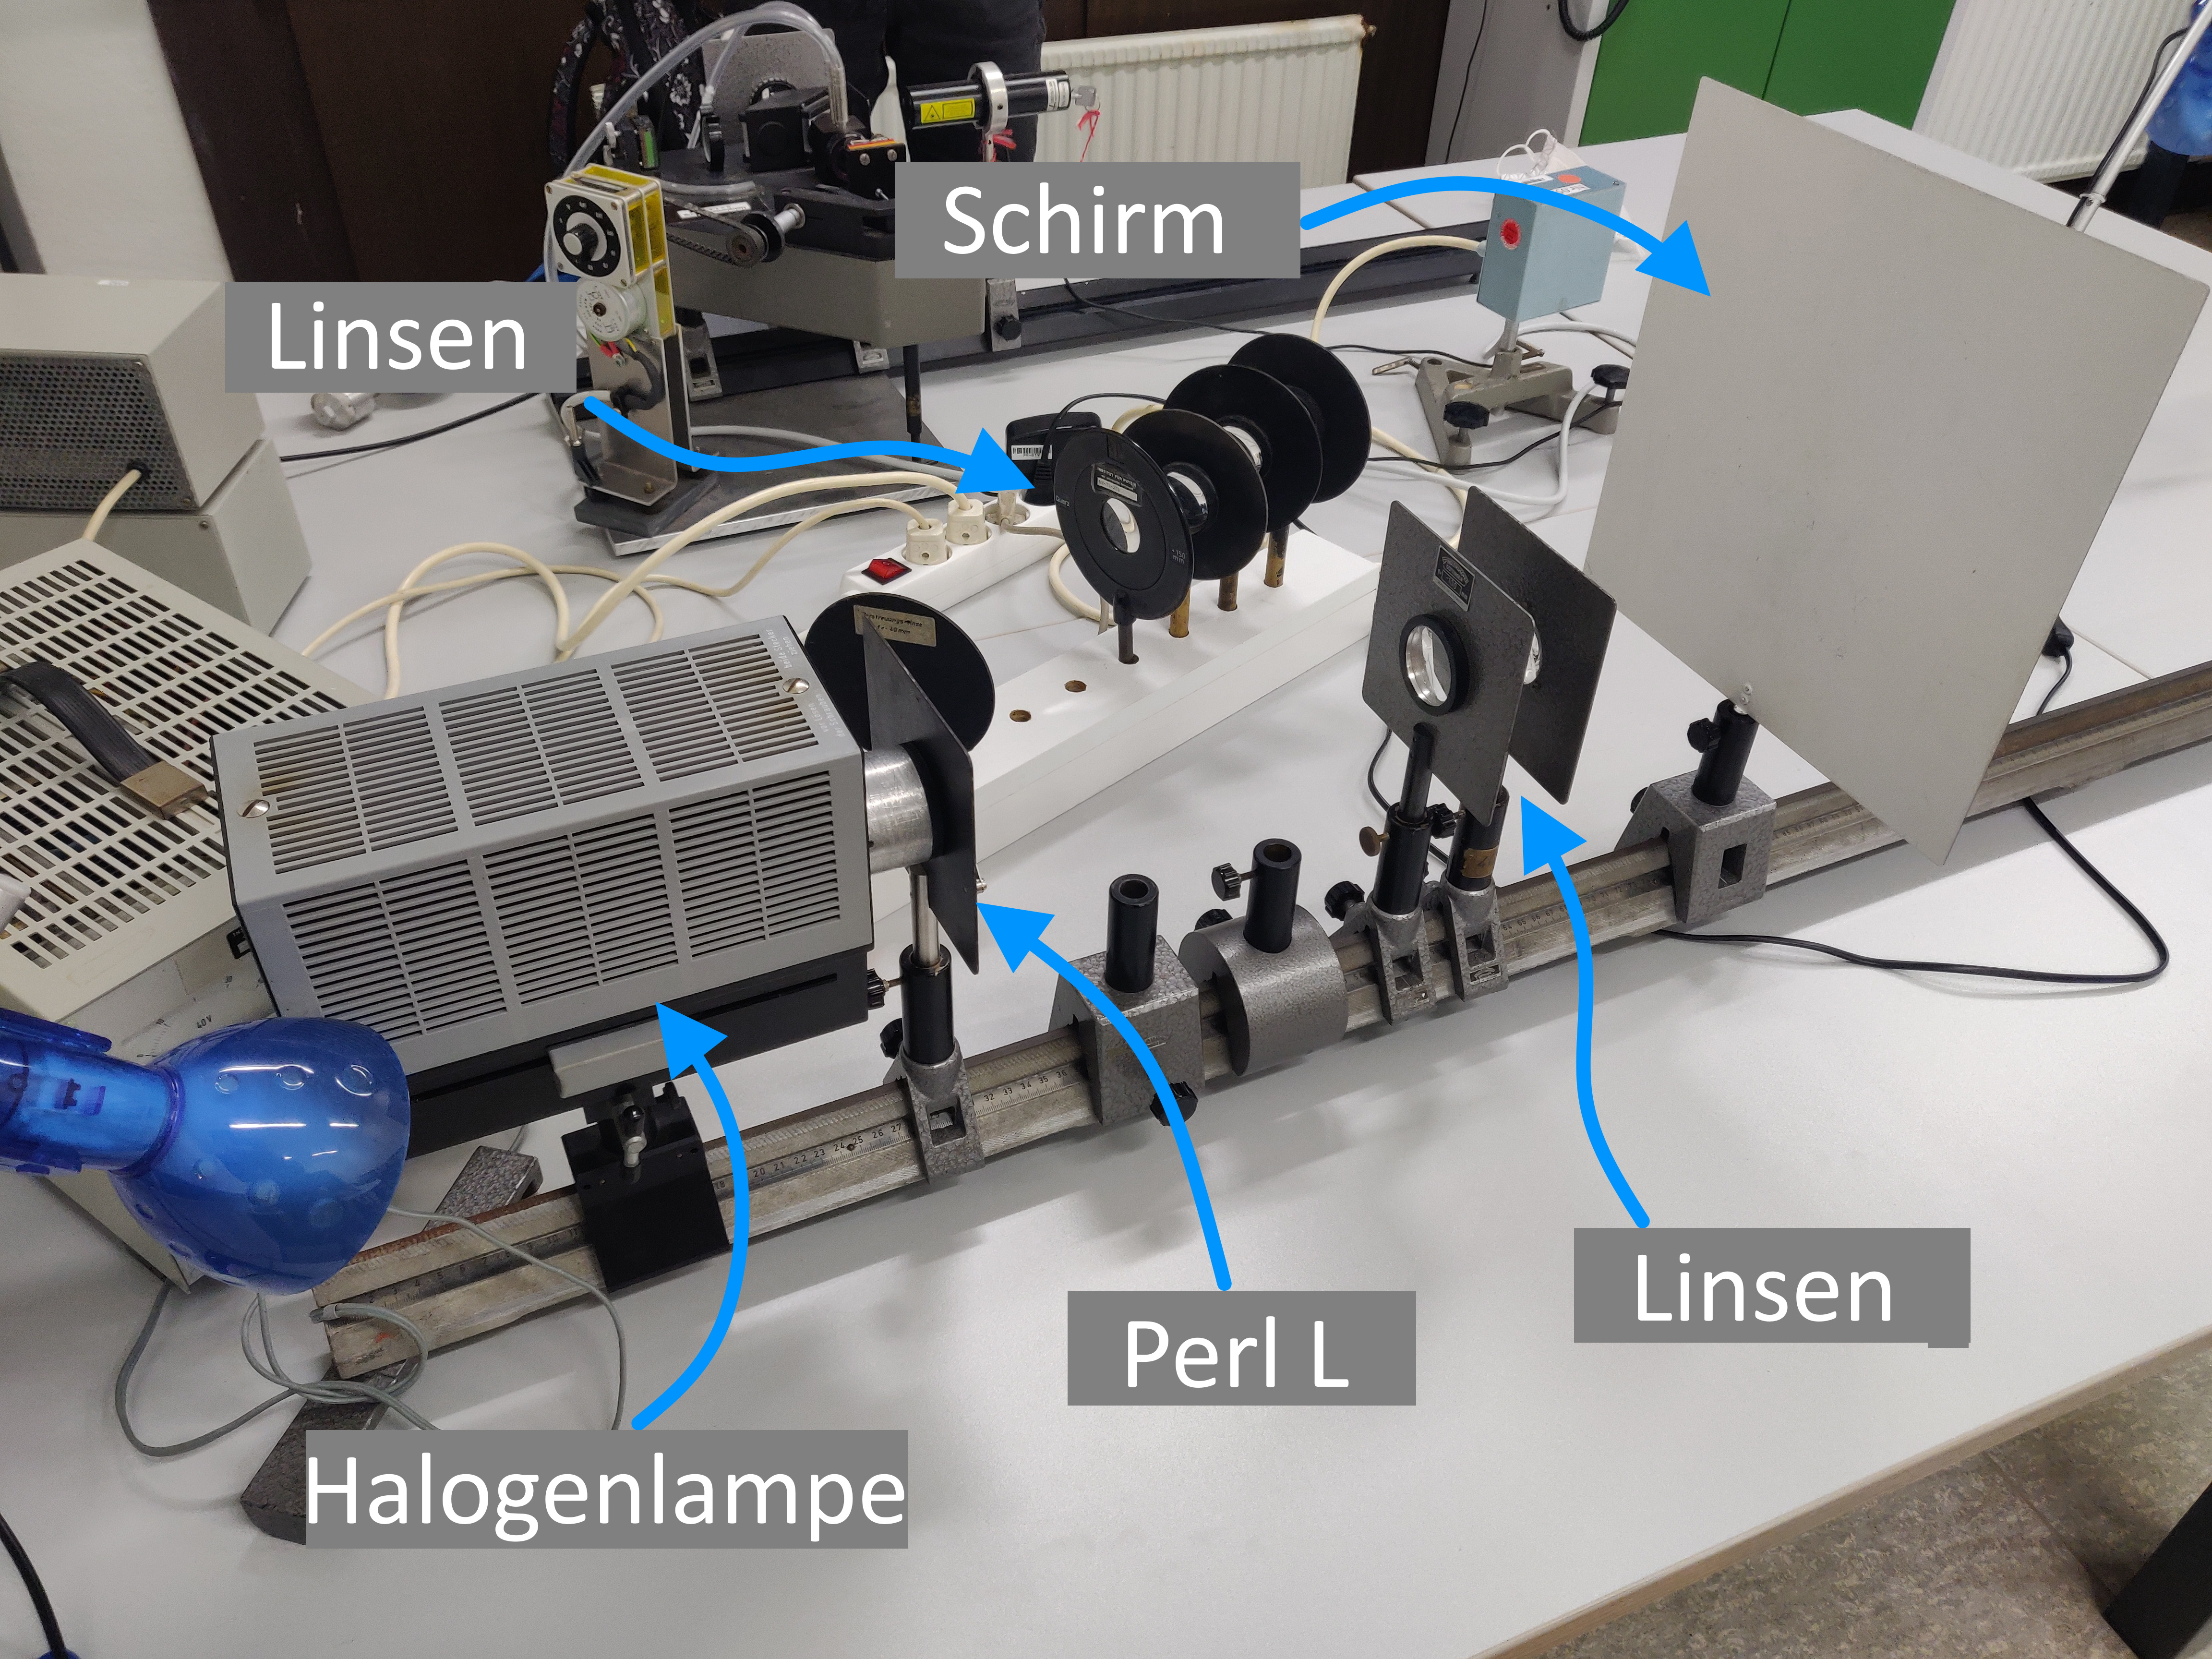
\includegraphics[width=.9\textwidth]{plots/VersuchRealB.jpg}
    \caption{Realer Versuchsaufbau.}
    \label{fig:VersuchReal}
\end{figure}

\begin{figure}
    \centering
    \includegraphics[width=.7\textwidth]{plots/PerlL.png}
    \caption{Modellhafte Darstellung der Schablone \textit{Perl L}.}
    \label{fig:PerlL}
\end{figure}

Das \textit{Perl L} wird direkt vor der Halogenlampe befestigt und die Position auf der optischen Bank notiert. Die Schablone wird anschließend für alle Messreihen nicht mehr bewegt.

\subsection{Aufbau -- Einfache Messreihe}
Für die erste Messreihe werden die optischen Elemente auf der Schiene befestigt und in ihrer Höhe aufeinander abgestimmt. Die Halogenlampe wird über einen Generator eingeschaltet und die Intensität an die
Lichtverhältnisse angepasst. Zudem wird die Lampe an der Austrittslinse durch entsprechendes Drehen scharfgestellt. Dies vereinfacht das Erkennen von Schärfe/Unschärfe im weiteren
Verlauf des Versuches.

Anschließend wird eine Sammellinse zwischen Schirm und Halogenlampe befestigt. Die Linse wird auf der Schiene hin- und her bewegt, bis das Bild \textit{L} auf dem Schirm scharf erscheint.
Die Position der Linse und des Schirms werden aufgeschrieben. Danach wird der Schirm beliebig verschoben. Daraufhin wird wieder die Linse verschoben, bis das Bild scharf ist.
Das Wertepaar wird notiert und dieser Vorgang insgesamt 10 Mal wiederholt. In einer Messreihe hat der Schirm niemals mehrfach dieselbe Position auf der Messschiene.

\subsection{Aufbau -- Methode von Bessel}
Für jede Linsenposition zwischen Schirm und Bilderzeuger gibt es zwei Punkte, an denen das Bild auf dem Schirm scharf wird. Für ein $f$ der Linsengleichung \eqref{eqn:Linsengleichung} bei dünnen Sammellinsen 
gibt es also stets zwei Lösungen für die gilt $b_1=g_2$ und $b_2=g_1$ (s. Abb. \ref{fig:Bessel}).
Für die Messreihe bedeutet das, dass der Schirm wieder in eine beliebige Position gebracht wird und durch Verschieben der Linse die beiden Fokuspunkte gefunden und die entsprechenden Wertepaare
notiert werden. Es werden für insgesamt 10 verschiedene Schirmpositionen Messungen durchgeführt.

\subsection{Aufbau -- Methode von Abbe}
Für diese Methode werden eine Sammellinse und eine Zerstreuungslinse mit den Brennweiten $\pm \SI{100}{\milli\meter}$ auf der Schiene befestigt und nah aneinander gestellt.
Die beiden Linsen brauchen einen kleinen Abstand zueinander, um scharfe Bilder zu erzeugen. Es empflieht sich, die Reiter so zu drehen, dass eine Verstellschraube eines Reiters zwischen
den beiden Halterungen ist und als Abstandshalter dient. Hierduch können beide Linsen gleichsam bewegt werden und den normierten Abstand beibehalten.
Für alle kommenden Messungen wird ein Referenzpunkt zwischen den beiden Linsen festgelegt, an dem die absolute Position auf der Messschiene abgelesen werden kann.
Danach wird die Schirmposition wie in der ersten Messreihe beliebig verstellt und das Bild über Verschiebung des Linsenpaares scharfgestellt. Für diese Methode kommt noch hinzu, dass die Größe des Bildes auf dem Schirm gemessen wird. Zu Beginn der Messreihe wird einmalig die Größe des \textit{Perl L} als Referenzwert gemessen.
Das Verschieben und Messen der Positionen wird insgesamt 10 Mal wiederholt.